\section*{Exercises 6.1}
%
\begin{enumerate}
\item Let  $f\x \mathbb{R} \to \mathbb{R}$ be defined by  $f\left( x \right) = x^2  - 2x$.
\begin{enumerate} \label{exer:sec61-2}
  \yitem Evaluate  $f( { - 3} ), f( { - 1} ), f( 1 ), \text{ and }f( 3 )$.

  \yitem Determine the set of all of the preimages of  0 and the set of all of the preimages of 4.

  %\item Determine all of the preimages of  $-2$.

  \item Sketch a graph of the function  $f$\!.

  \yitem Determine the range of the function  $f$\!.
\end{enumerate}

\item Let  
$\mathbb{R}^*  = \left\{ { {x \in \mathbb{R}} \mid x \geq 0} \right\}$, and let  
$s\x \mathbb{R} \to \mathbb{R}^* $ be defined by  $s( x ) = x^2 $.

\begin{enumerate}
  \item Evaluate  $s( { - 3} ), s( { - 1} ), s( 1 ), \text{ and }s( 3 )$.

  \item Determine the set of all of the preimages of  0 and the set of all preimages of 2.

  \item Sketch a graph of the function  $s$.

  \item Determine the range of the function  $s$.

\end{enumerate}

%\item Let  $A = \left\{ {1, 2, 3, 4} \right\}$ and let  $B = \left\{ {a, b, c} \right\}$.  Which of the following arrow diagrams can be used to represent a function from  $A$  to  $B$?  Explain. \label{exer:sec61-1}
%
%\begin{multicols}{2}
%\begin{figure}[h]
%\begin{center}
%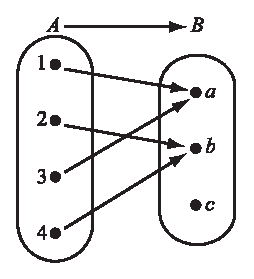
\includegraphics{figps-arrow-exer611.eps} 
%\caption{Arrow Diagram for a Function} \label{fig:arrow61-1}
%\end{center}
%\end{figure}
%
%\begin{figure}[h]
%\begin{center}
%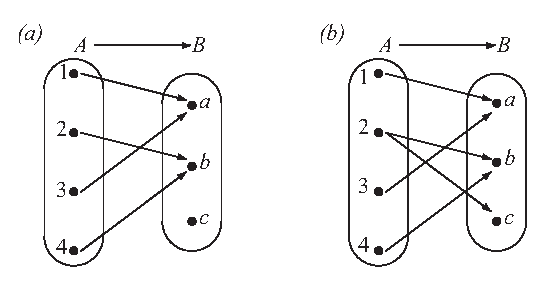
\includegraphics{figps-arrow-exer611ab.eps} 
%\caption{Arrow Diagram for a Function} \label{fig:arrow61-1}
%\end{center}
%\end{figure}
%
%\begin{figure}[h]
%\begin{center}
%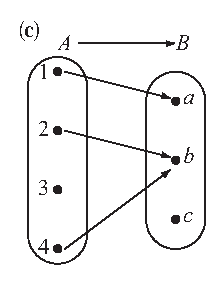
\includegraphics{figps-arrow-exer611c.eps} 
%\caption{Arrow Diagram for a Function} \label{fig:arrow61-1}
%\end{center}
%\end{figure}
%\end{multicols}

\item Let  $f\x \mathbb{Z} \to \mathbb{Z}$ be defined by  $f( m ) = 3 - m$. \label{exer61:integerfunction}

\begin{enumerate}
  \yitem Evaluate  $f( { - 7} ), f( { - 3} ), f( 3 ), \text{ and }f( 7 )$.

  \yitem Determine the set of all of the preimages of  5 and the set of all of the preimages of 4. 

  \yitem Determine the range of the function  $f$\!.

  \item This function can be considered a real function since  $\Z \subseteq \R$.  Sketch a graph of this function. \note The graph will be an infinite set of points that lie on a line.  However, it will not be a line since its domain is not $\R$ but is $\Z$. 
\label{exer:sec61-real}
\end{enumerate}

\item Let  $f\x \mathbb{Z} \to \mathbb{Z}$ be defined by $f( m ) = 2m + 1$. \label{exer:sec61-5}

\begin{enumerate}
 \item Evaluate  $f( { - 7} ), f( { - 3} ), f( 3 ), \text{ and }f( 7 )$.

  \yitem Determine the set of all of the preimages of  5 and the set of all of the preimages of 4.

  \yitem Determine the range of the function  $f$\!.

  \yitem Sketch a graph of the function  $f$.  See the comments in Exercise~(\ref{exer:sec61-real}).
\end{enumerate}


%\newpage
%\xitem Let $f\x \mathbb{Z} \times \mathbb{Z} \to \mathbb{Z}$ be defined by  
%$f( {m, n} ) = m + 3n$. \label{exer:sec61-7}
%
%\begin{enumerate}
%  \item Calculate  $f( { - 3, 4} )$ and  $f( { - 2, - 7} )$.
%
%  \item Determine the set of all the preimages of  4 by using set builder notation to describe the set of all $\left( {m, n} \right) \in \mathbb{Z} \times \mathbb{Z}$ such that  
%$f( {m, n} ) = 4$.
%\end{enumerate}

%\item Let $g\x \mathbb{Z} \times \mathbb{Z} \to \mathbb{Z} \times \mathbb{Z}$ be defined by  
%$g( {m, n} ) = \left( {2m, m - n} \right)$.  
%\label{exer:sec61-8}%
%
%\begin{enumerate}
%  \item Calculate  $g( {3, 5} )$ and  $g( { - 1, 4} )$.
%
%  \item Determine all the preimages of  $\left( {0, 0} \right)$.  That is, find all  
%$( {m, n} ) \in \mathbb{Z} \times \mathbb{Z}$ such that  $g( {m, n} ) = ( {0, 0} )$.
%
%  \item Determine the set of all the preimages of  $( {8,  - 3} )$.
%
%  \item Determine the set of all the preimages of  $( {1, 1} )$.
%
%  \item Is the following proposition true or false?  Justify your conclusion.
%  \begin{list}{}
%  \item For each  $( {s, t} ) \in \mathbb{Z} \times \mathbb{Z}$, there exists an $( {m, n}) \in \mathbb{Z} \times \mathbb{Z}$ such that  $g( {m, n} ) = ( {s, t} )$.
%  \end{list}
%\end{enumerate}

\item Recall that a \textbf{real function}
\index{real function}%
\index{function!real}%
 is a function whose domain and codomain are subsets of the real numbers  $\R$.  (See page~\pageref{realfunction}.)  Most of the functions used in calculus are real functions.  Quite often, a real function is given by a formula or a graph with no specific reference to the domain or the codomain.  In these cases, the usual convention is to assume that the domain of the real function  $f$  is the set of all real numbers  $x$  for which  $f( x )$  is a real number, and that the codomain is  
$\mathbb{R}$.  For example, if we define the (real) function  $f$  by  
\[
f( x ) = \frac{x}{{x - 2}},
\]
we would be assuming that the domain is the set of all real numbers that are not equal to  2 and that the codomain is $\R$.  
%That is, we would be assuming that  \\$\text{dom}\left( f \right) = \left\{ {x \in \mathbb{R}
% \, \mid x \ne 2} \right\}$.

Determine the domain and range of each of the following real functions. \label{exer:sec61-9}  It might help to use a graphing calculator to plot a graph of the function.

\begin{enumerate}
  \item The function  $k$  defined by  $k( x ) = \sqrt {x - 3} $

  \yitem The function  $F$  defined by  $F( x ) = \ln \left( {2x - 1} \right)$

  \item The function  $f$  defined by  $f( x ) = 3\sin( {2x} )$

  \yitem The function  $g$ defined by  $g( x ) = \dfrac{4}{{x^2  - 4}}$

  \item The function $G$ defined by $G(x) = 4 \cos \left( \pi x \right) + 8$
\end{enumerate}


\xitem \textbf{The number of divisors function}.\label{exer:numberofdivisors}
\index{number of divisors function}%
  Let  $d$  be the function that associates with each natural number the number of its natural number divisors.  That is,  $d\x \mathbb{N} \to \mathbb{N}$  where  $d( n )$  
\label{sym:numdivisors} is the number of natural number divisors of  $n$.  For example,  
$d( 6 ) = 4$ since  1, 2, 3, and  6  are the natural number divisors of  6.

\begin{enumerate}
  \item Calculate  $d( k )$  for each natural number  $k$  from  1  through  12.

  \item Does there exist a natural number  $n$  such that  $d( n ) = 1$?  What is the set of preimages of the natural number  1?

  \item Does there exist a natural number  $n$  such that  $d( n ) = 2$? If so, determine the set of all preimages of the natural number  2.

  \item Is the following statement true or false?  Justify your conclusion.
  \begin{center}
  For all  $m, n \in \mathbb{N}$, if $m \ne n$, then  $d( m ) \ne d( n )$.
  \end{center}

  \item Calculate  $d\!\left( {2^k } \right)$ for  $k = 0$ and for each natural number  $k$  from  1 through 6.  \label{exer:numberofdivisorse}

  \item Based on your work in Exercise~(\ref{exer:numberofdivisorse}), make a conjecture for a formula for  $d\!\left( {2^n } \right)$ where $n$ is a nonnegative integer.  Then explain why your conjecture is correct.

  \item Is the following statement is true or false?
  \begin{list}{}
  \item For each  $n \in \mathbb{N}$, there exists a natural number  $m$  such that  \linebreak
$d( m ) = n$.
  \end{list}
\end{enumerate}


\item In Exercise~(\ref{exer:numberofdivisors}), %from Section~\ref{S:introfunctions}, 
we introduced the \textbf{number of divisors function}
\index{number of divisors function}%
  $d$.  For this function, $d\x \mathbb{N} \to \mathbb{N}$,
where  $d( n )$ is the number of natural number divisors of  $n$.  

A function that is related to this function is the so-called \textbf{set of divisors function}.
\index{set of divisors function}%
  This can be defined as a function  $S$  that associates with each natural number the set of its distinct natural number factors.  For example,  
$S( 6 ) = \left\{ {1, 2, 3, 6} \right\}$ and $S(10) = \{1, 2, 5, 10 \}$. \label{exer:sec62-5}

\begin{enumerate}
\yitem Discuss the function  $S$  by carefully stating its domain, codomain, and its rule for determining outputs.

\yitem Determine  $S( n )$  for at least five different values of  $n$.

\yitem Determine  $S( n )$  for at least three different prime number values of  $n$.

\item Does there exist a natural number  $n$  such that  
$\card (S(n)) = 1$?  Explain.  [Recall that  $\card (S(n))$ is the number of elements in the set  
$S( n )$.]

\item Does there exist a natural number  $n$  such that  $\card (S(n)) = 2$?  Explain.

\item Write the output for the function  $d$  in terms of the output for the function  $S$.  That is, write  $d( n )$  in terms of  $S( n )$.

\item Is the following statement true or false?  Justify your conclusion.
\begin{list}{}
\item For all natural numbers $m$ and $n$, if $m \ne n$, then 
$S ( m ) \ne S ( n )$.
\end{list}

\item Is the following statement true or false?  Justify your conclusion.
\begin{list}{}
\item For all sets $T$ that are subsets of $\mathbb{N}$, there exists a natural number $n$ such that $S( n ) = T$.
\end{list}
\end{enumerate}

\end{enumerate}

\subsection*{Explorations and Activities}
%\newcounter{oldenumi}
\setcounter{oldenumi}{\theenumi}
\begin{enumerate} \setcounter{enumi}{\theoldenumi}
  \item \textbf{Creating Functions with Finite Domains}. Let  $A = \left\{ {a,b,c,d} \right\}$, $B = \left\{ {a,b,c} \right\}$, and  
$C = \left\{ {s,t,u,v} \right\}$.  In each of the following exercises, draw an arrow diagram to represent your function when it is appropriate.
\begin{enumerate}
\item Create a function  $f\x A \to C$ whose range is the set   $C$  or explain why it is not possible to construct such a function.

\item Create a function  $f\x A \to C$ whose range is the set  $\left\{ {u, v} \right\}$ or explain why it is not possible to construct such a function.

\item Create a function  $f\x B \to C$ whose range is the set   $C$  or explain why it is not possible to construct such a function.

\item Create a function  $f\x A \to C$ whose range is the set  $\left\{ u \right\}$ or explain why it is not possible to construct such a function.

\item If possible, create a function  $f\x A \to C$  that satisfies the following condition:
\begin{list}{}
\item For all  $x, y \in A$,  if  $x \ne y$, then  $f( x ) \ne f( y )$.
\end{list}
If it is not possible to create such a function, explain why.

\item If possible, create a function  $f\x A \to \left\{ {s, t, u} \right\}$ that satisfies the following condition:

\begin{list}{}
\item For all  $x, y \in A$,  if  $x \ne y$, then  $f( x ) \ne f( y )$.
\end{list}

If it is not possible to create such a function, explain why.
\end{enumerate}




%\item \textbf{Derivatives of Even and Odd Functions}.  Certain types of real functions are given names.  A function $g \x \R \to \R$ is called an \textbf{even function} 
%\index{even function}%
%\index{function!even}%
%provided that for each $x \in \R$, $g(-x) = g(x)$, and a function $h \x \R \to \R$ is called an \textbf{odd function}  
%\index{odd function}%
%\index{function!odd}%
%provided that for each $x \in \R$, $h(-x) = - h(x)$.  For example,
%\[
%f \x \R \to \R  \text{ by } f(x) = 2x^4 - x^2
%\]
%is an even function since for each $x \in \R$,
%\begin{align*}
%f(-x) &= 2(-x)^4 - (-x)^2 \\
%     &= 2x^4 - x^2 \\
%     &= f(x).
%\end{align*}
%Notice that $f'(x) = 8x^3 - 2x$.  So the derivative function is $f' \x \R \to \R$ where $f'(x) = 8x^3 - 2x$.  Notice that for each $x \in \R$,
%\begin{align*}
%f'(-x) &= 8(-x)^3 - 2(-x) \\
%       &= 8(-x^3) - (-2x) \\
%       &= -8x^3 + 2x \\
%       &= - f'(x).
%\end{align*}
%Hence, the derivative function $f'$ is an odd function.
%
%In addition, the trigonometric identities $\cos (-x) = \cos x$ and $\sin (-x) = -\sin x$ for each $x \in \R$ imply that the cosine function is an even function and the sine function is an odd function.
%\begin{enumerate}
%  \item Explain why the function $f \x \R \to \R$, where $f(x) = \cos x + 2$ for each $x \in \R$, is neither an even function or an odd function.
%  \item Is the following proposition true or false?  Justify your conclusion.
%\begin{list}{}
%\item Let $f \x \R \to \R$ be a differentiable function.  If $f$ is an even function, then its derivative $f'$ is an odd function.
%\end{list}
%  \item Is the following proposition true or false?  Justify your conclusion.
%\begin{list}{}
%\item Let $f \x \R \to \R$ be a differentiable function.  If $f'$ is an odd function and $f(0) = 0$, then $f$ is an even  function.
%\end{list}
%  \item Is it possible to find a differentiable function $f \x \R \to \R$ such that $f$ is not an even function but its derivative $f'$ is an odd function?  Justify your conclusion.
%
%\end{enumerate}

\end{enumerate}


\hbreak
%\markboth{Chapter~\ref{C:functions}. Functions}{\ref{S:moreaboutfunctions}. More about Functions}
\endinput


\begin{enumerate}  \item 
\begin{multicols}{2}
\setlength{\unitlength}{0.25cm}
\begin{picture}(14,18)
\put(2,8){\oval(4,14)}
\put(10,8){\oval(4,12)}

\put(2,2){\circle*{.5}}
\put(2,6){\circle*{.5}}
\put(2,10){\circle*{.5}}
\put(2,14){\circle*{.5}}

\put(10,4){\circle*{.5}}
\put(10,8){\circle*{.5}}
\put(10,12){\circle*{.5}}

\put(1.1,13.8){1}
\put(1.1,9.8){2}
\put(1.1,5.8){3}
\put(1.1,1.8){4}
\put(10.5,11.8){$a$}
\put(10.5,7.8){$b$}
\put(10.5,3.8){$c$}

\put(2,15.5){$A$}
\put(10,15.5){$B$}

\put(3.4,15.9){\vector(1,0){6.5}}

\put(2.5,2){\vector(4,3){7.1}}
\put(2.5,6){\vector(4,3){7.1}}
\put(2.5,10){\vector(4,-1){7.1}}
\put(2.5,14){\vector(4,-1){7.1}}

\end{picture}

\item 
\setlength{\unitlength}{0.25cm}
\begin{picture}(14,18)
\put(2,8){\oval(4,14)}
\put(10,8){\oval(4,12)}

\put(2,2){\circle*{.5}}
\put(2,6){\circle*{.5}}
\put(2,10){\circle*{.5}}
\put(2,14){\circle*{.5}}

\put(10,4){\circle*{.5}}
\put(10,8){\circle*{.5}}
\put(10,12){\circle*{.5}}

\put(1.1,13.8){1}
\put(1.1,9.8){2}
\put(1.1,5.8){3}
\put(1.1,1.8){4}
\put(10.5,11.8){$a$}
\put(10.5,7.8){$b$}
\put(10.5,3.8){$c$}

\put(2,15.5){$A$}
\put(10,15.5){$B$}

\put(3.4,15.9){\vector(1,0){6.5}}

\put(2.5,2){\vector(4,3){7.1}}
\put(2.5,6){\vector(4,3){7.1}}
\put(2.5,10){\vector(4,-1){7.1}}
\put(2.5,10){\vector(4,-3){7.1}}
\put(2.5,14){\vector(4,-1){7.1}}

\end{picture}
\end{multicols}

\item 
\begin{center}
\setlength{\unitlength}{0.25cm}
\begin{picture}(14,18)
\put(2,8){\oval(4,14)}
\put(10,8){\oval(4,12)}

\put(2,2){\circle*{.5}}
\put(2,6){\circle*{.5}}
\put(2,10){\circle*{.5}}
\put(2,14){\circle*{.5}}

\put(10,4){\circle*{.5}}
\put(10,8){\circle*{.5}}
\put(10,12){\circle*{.5}}

\put(1.1,13.8){1}
\put(1.1,9.8){2}
\put(1.1,5.8){3}
\put(1.1,1.8){4}
\put(10.5,11.8){$a$}
\put(10.5,7.8){$b$}
\put(10.5,3.8){$c$}

\put(2,15.5){$A$}
\put(10,15.5){$B$}

\put(3.4,15.9){\vector(1,0){6.5}}

\put(2.5,2){\vector(4,3){7.1}}
%\put(2.5,6){\vector(4,3){7.1}}
\put(2.5,10){\vector(4,-1){7.1}}
\put(2.5,14){\vector(4,-1){7.1}}

\end{picture}
\end{center}

\end{enumerate}

